\documentclass{standalone}
\begin{document}
	\begin{frame}{Basic Idea}{Colour Quantization for Medical Image Segmentation}
		
		\begin{columns}
			\begin{column}{.4\textwidth}
				\begin{block}{GGO areas on CT Images}
					\begin{itemize}
						\item Similar Gray Level
						\item Spatially Displaced
					\end{itemize}				
				\end{block}
				\begin{block}{Basic Idea}
					\begin{itemize}
						\item \textbf{Colour Quantization}: Group Pixel Based on colour similarity
						\item \textbf{Colour Space}: Constructed by taking into accounts different information
					\end{itemize}
				\end{block}				
			\end{column}
			\begin{column}{.5\textwidth}
				\centering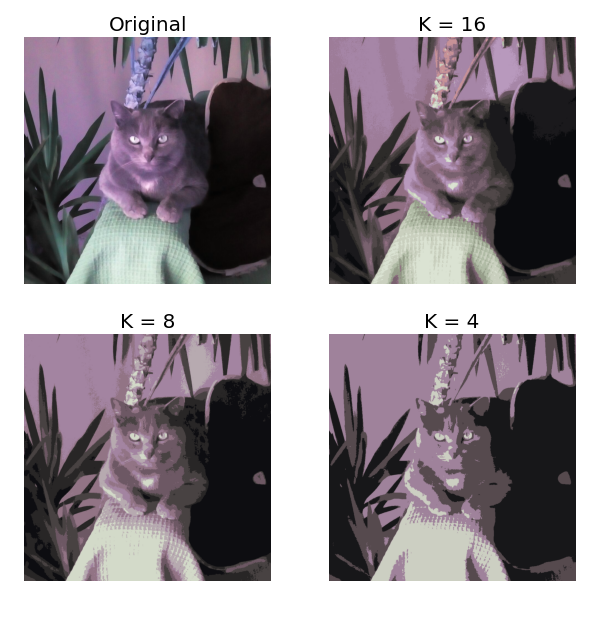
\includegraphics[width=\linewidth]{./img/ColorQuantization}
			\end{column}
		\end{columns}
	\end{frame}
\end{document}